\lecture{2}{28. August 2025}{Moment of a force}

\subsection{Dot product}
The dot product of vectors $\textbf{A}$ and $\textbf{B}$ is defined as:
\[ 
\textbf{A}\cdot \textbf{B} = AB \cos \theta
.\]
This is also called the scalar product of the vectors. The following laws of operation apply:
\begin{align*}
  \textbf{A} \cdot \textbf{B} &= \textbf{B} \cdot \textbf{A} \\
  a \left( \textbf{A} \cdot \textbf{B} \right) &= \left( a \textbf{A} \right) \cdot \textbf{B} = \textbf{A} \cdot \left( a \textbf{B} \right) \\
  \textbf{A} \cdot \left( \textbf{B} + \textbf{D} \right) &= \left( \textbf{A} \cdot \textbf{B} \right) + \left( \textbf{A} \cdot \textbf{D} \right)
.\end{align*}

In Cartesian form the dot product can be expressed as:
\[ 
\textbf{A} \cdot \textbf{B} = A_x B_x + A_y B_y + A_z B_z
.\]


\section{Force system resultants}

\subsection{Moment of a force – Scalar formulation}
A force applied to a body will tend to produce a rotation about a point that is not on the line of action of the force -- this phenomenon is called the \textit{moment} or the \textit{torque}. 

In general, if we consider the force $\textbf{F}$ and point $O$ to lie in the shaded plane shown on \textbf{\autoref{fig:f3_2}}, then the moment $\textbf{M}_O$ about the point $O$, or about an axis through $O$ and perpendicular to the plane is a vector quantity since it has both a magnitude and a direction.

\begin{figure} [ht]
  \centering
  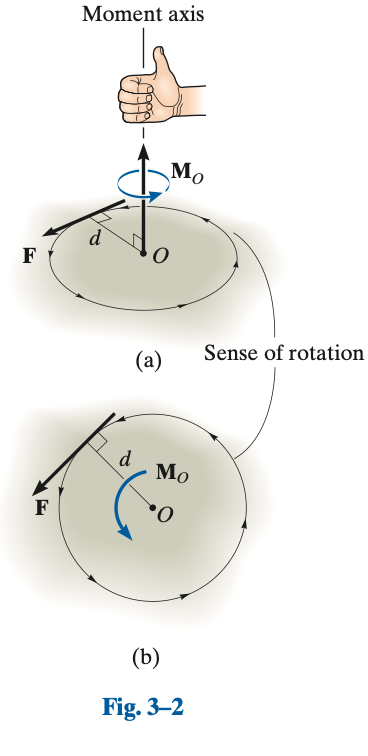
\includegraphics[width=0.25\linewidth]{./figures/f3_2.png}
  \caption{}
  \label{fig:f3_2}
\end{figure}

The magnitude of $\textbf{M}_O$ is
\[ 
  M_O = Fd
\]
where $d$ is the \textit{moment arm} or the perpendicular distance from the axis through point $O$ to the line of action of the force. 

The direction of $\textbf{M}_O$ can be determined using the right hand rule -- curl the fingers in the direction of rotation and the thumb will be pointing in the direction of the moment.

The resultant moment of multiple forces lying in the same plane is simply found by their algebraic sum. I.e.
\[ 
M_{R_O} = \sum F d
.\]

\subsection{Principle of moments}
A very useful concept often used in mechanics is the principle of moments, which is also known as Varignon's theorem.

\begin{definition}[Principle of moments]
  The moment of a force about a point is equal to the sum of the moments of the components of the force about the point.
\end{definition}

\begin{figure} [ht]
  \centering
  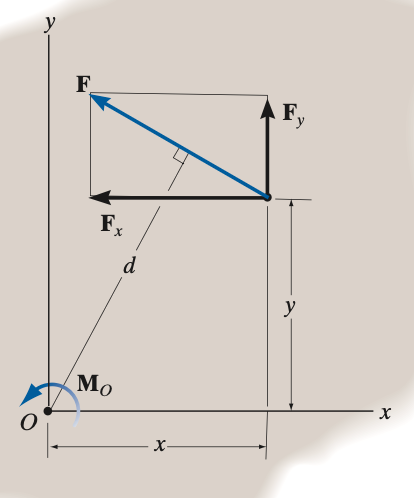
\includegraphics[width=0.35\linewidth]{./figures/f3_4.png}
  \caption{}
  \label{fig:f3_4}
\end{figure}

This can be applied to the case shown on \textbf{\autoref{fig:f3_4}}. Here a force $\textbf{F}$ is split into components and the resultant moment can then simply be found as:
\[ 
M_O = F_x y + F_y x
.\]

\subsection{Cross product}
The cross product of the two vectors $\textbf{A}$ and $\textbf{B}$ yields a vector $\textbf{C}$ as:
\[ 
\textbf{C} = \textbf{A} \times \textbf{B}
.\]

The magnitude of $\textbf{C}$ is given by:
\[ 
C = AB \sin \theta
.\]

The vector $\textbf{C}$ will have a direction perpendicular to the plane containing $\textbf{A}$ and $\textbf{B}$ according to the right hand rule.

The following laws of operation apply:
\begin{align*}
  \textbf{A} \times \textbf{B} &= - \textbf{B} \times \textbf{A} \\
  a \left( \textbf{A} \times \textbf{B} \right) &= (a \textbf{A}) \times \textbf{B} = \textbf{A} \times \left( a \textbf{B} \right) \\
  \textbf{A} \times \left( \textbf{B} + \textbf{D} \right) &= \left( \textbf{A} \times \textbf{B} \right) + \left( \textbf{A} \times \textbf{D} \right)
.\end{align*}

In Cartesian coordinates the cross product may be written as:
\[ 
\textbf{A} \times \textbf{B} = \left( A_y B_z - A_z B_y \right) \textbf{i} - \left( A_x B_z - A_z B_x \right) \textbf{j} + \left( A_x B_y - A_y B_x \right) \textbf{k}
.\]

In determinant form it is:
\[ 
\textbf{A} \times \textbf{B} = \left| \begin{array}{ccc}
\textbf{i} & \textbf{j} & \textbf{k}\\
A_x & A_y & A_z\\
B_x & B_y & B_z\\
\end{array} \right|
.\]

\subsection{Moment of a force -- Vector formulation}
The moment of a force $\textbf{F}$ about point $O$ can be expressed using the vector cross product as:
\[ 
\textbf{M}_O = \textbf{r} \times \textbf{F}
.\]
Here $\textbf{r}$ is a position vector \textit{from} $O$ \textit{to any point} on the line of action of $\textbf{F}$. When using this formulation $\textbf{M}_O$ will have the correct magnitude and direction no matter what position vector is chosen along as the previous rule is respected.

The magnitude of this is:
\[ 
M_O = r F \sin \theta = F \left( r \sin \theta \right) = Fd
\]
and the direction of $\textbf{M}_O$ is once again determined by the right hand rule. 

The cross product is typically used in three dimensions since the perpendicular distance or moment arm from point $O$ to the line of action of the force is not needed. In other words any position vector $\textbf{r}_i$ pointing from the point $O$ to the line of action of $\textbf{F}$ is adequate. 

If a body is acted upon by a system of forces, the resultant moment of the forces about point $O$ can be determined by vector addition of the moment of each force as:
\[ 
\textbf{M}_{R_O} = \sum \left( \textbf{r} \times \textbf{F} \right)
.\]


\subsection{Moment of a couple}
A \textit{couple} is defined as two parallel forces that hav equal magnitude but opposite directions and are separated by a distance $d$ as shown on \textbf{\autoref{fig:f3_25}}. Since the resultant force of the couple is zero the only effect is to produce a tendency for rotation.

\begin{figure} [ht]
  \centering
  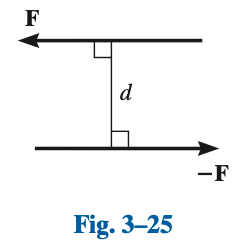
\includegraphics[width=0.25\linewidth]{./figures/f3_25.png}
  \caption{}
  \label{fig:f3_25}
\end{figure}

The moment produced by a couple is called a \textit{couple moment} it can be shown that this is equal to:
\[ 
\textbf{M} = \textbf{r} \cdot \textbf{F}
.\]
This is a \textit{free vector}, i.e. it can act at \textit{any point} since $\textbf{M}$ only depends on the position vector $r$ between the forces and not the position vectors from the origin.


\subsection{Simplification of a force and couple system}
It is often convenient to reduce a complex system of forces and couple moments acting on a body to a simpler form by replacing it with an equivalent system. A system is equivalent if the \textit{external effects} it produces on a body are the same as those caused by the original force and moment system. 

Every system of several forces and couple moments can be broken down into a single resultant force acting at a point $O$ and a resultant couple moment. This can be done by adding together the forces in each Cartesian direction as well as the moments each on their own. 

\subsection{Reduction of a simple distributed loading}
Sometimes, a body is subjected to a load distributed over its surface. The pressure caused by this distributed loading on the surface represents the loading intensity and is measured in \unit{Pa}. 

The most common type of distributed loading is that along a single axis. Take for example a beam of constant width $b$ subjected to a pressure loading that varies along the $x$-axis. The loading is described by the function $p = p(x)$. Since this contains only one variable we can quickly ``one-dimensionalize'' the problem by $w(x) = p(x) b$. 

The magnitude of the resultant force in this case must be found using integration as summing ``all the forces'' would require an infinte sum. I.e.
\[ 
F_R = \int_{L} w(x) \, \mathrm{d}x = \int_A \, \mathrm{d}A = A
.\]
The location $\overline{x}$ of $\textbf{F}_R$ can be determined using static equilibrium and moments as:
\[ 
- \overline{x} F_R = - \int_L x w(x) \, \mathrm{d}x 
.\]
And solving for $\overline{x}$ we have:
\[ 
\overline{x} = \frac{\int_L x w (x) \, \mathrm{d}x}{\int_L w(x) \, \mathrm{d}x} = \frac{\int_A x \, \mathrm{d}A}{\int_A \, \mathrm{d}A}
.\]
